% =============================================================================
% Rapport de projet académique — VisioFind
% Compilation recommandée : pdflatex (2 passes) ou latexmk -pdf
% Répertoire de travail : dossier docs/ (les captures sont dans ./screenshots/)
% =============================================================================
\documentclass[11pt,a4paper,openany]{report}

\usepackage[utf8]{inputenc}
\usepackage[T1]{fontenc}
\usepackage[french]{babel}
\addto\captionsfrench{\renewcommand{\listfigurename}{Liste des figures}}
\usepackage{csquotes}
\usepackage{amsmath,amssymb}
\usepackage{geometry}
\geometry{margin=2.5cm}
\usepackage{setspace}
\onehalfspacing
\usepackage{microtype}

\usepackage{hyperref}
\hypersetup{
  colorlinks=true,
  linkcolor=blue!60!black,
  urlcolor=blue!70!black,
  citecolor=blue!60!black,
  pdftitle={VisioFind — Rapport de projet},
  pdfauthor={Équipe projet VisioFind}
}

\usepackage{graphicx}
% Tolère la compilation depuis docs/ ou depuis la racine du projet.
\graphicspath{{screenshots/}{./screenshots/}{docs/screenshots/}{./docs/screenshots/}}
\usepackage{float}
\usepackage{caption}
\usepackage{subcaption}
\captionsetup{font=small, labelfont=bf}

\usepackage{booktabs}
\usepackage{longtable}
\usepackage{array}
\usepackage{enumitem}
\usepackage{xcolor}
\usepackage{listings}

\usepackage{tikz}
\usetikzlibrary{arrows.meta,positioning,fit,shapes.multipart,calc}

% --- Code listings ---
\definecolor{codegreen}{rgb}{0,0.45,0}
\definecolor{codegray}{rgb}{0.45,0.45,0.45}
\lstset{
  language=Python,
  basicstyle=\ttfamily\footnotesize,
  keywordstyle=\color{blue!70!black},
  commentstyle=\color{codegray},
  stringstyle=\color{codegreen},
  breaklines=true,
  frame=single,
  rulecolor=\color{black!30},
  tabsize=4,
  showstringspaces=false,
  columns=fullflexible
}

% --- Métadonnées (à personnaliser) ---
\newcommand{\NomUniversite}{Université --- Département ---}
\newcommand{\NomCours}{Cours / Module d'intelligence artificielle et vision}
\newcommand{\AuteursRapport}{Présenté par : Majda Rane, Ayoub Elkarkoub}
\newcommand{\Encadrant}{Anouar Ben-Loghfery}

\begin{document}

% =============================================================================
% 1. PAGE DE GARDE
% =============================================================================
\begin{titlepage}
  \singlespacing
  \noindent
  \begin{minipage}[t]{0.45\textwidth}
    \raggedright
    \includegraphics[height=2.5cm]{screenshots/logo_fst.png}
  \end{minipage}%
  \hfill
  \begin{minipage}[t]{0.45\textwidth}
    \raggedleft
    \includegraphics[height=2.5cm]{screenshots/logo_uh2.png}
  \end{minipage}

  \vspace*{1.5cm}
  \centering

  {\Large\NomUniversite\par}
  \vspace{0.8cm}
  {\large\NomCours\par}
  \vspace{2.5cm}
  \rule{\textwidth}{1.5pt}\\[0.6cm]
  {\Huge\bfseries VisioFind\par}
  \vspace{0.4cm}
  {\LARGE Recherche visuelle par apprentissage profond\par}
  \vspace{0.3cm}
  {\large Objets, animaux, lieux — Images, vidéo et cartographie\par}
  \rule{\textwidth}{1.5pt}\\[2cm]
  {\Large\textbf{Rapport de projet}\par}
  \vspace{1.5cm}
  {\large\AuteursRapport\par}
  \vspace{0.5cm}
  {\normalsize Encadrant : \Encadrant\par}
  \vfill
  {\large Année universitaire \the\year\par}
  \vspace{1cm}
\end{titlepage}

% =============================================================================
% 2. REMERCIEMENTS
% =============================================================================
\chapter*{Remerciements}
\addcontentsline{toc}{chapter}{Remerciements}

Nous adressons nos remerciements à \Encadrant{} pour l'encadrement, les orientations méthodologiques et les retours critiques tout au long de ce travail. Nous remercions également les enseignants du département pour les enseignements en traitement du signal, en vision par ordinateur et en apprentissage profond qui ont constitué les bases théoriques de ce projet. Enfin, nous salutations la communauté scientifique et open source (OpenAI, Hugging Face, les mainteneurs de Streamlit et PyTorch) sans laquelle la réalisation d'un tel prototype serait nettement plus coûteuse en temps et en ressources.

\cleardoublepage

% =============================================================================
% 3. RÉSUMÉ (FR) + ABSTRACT (EN)
% =============================================================================
\chapter*{Résumé}
\addcontentsline{toc}{chapter}{Résumé}

\textbf{Mots-clés :} recherche visuelle, apprentissage profond, CLIP, traitement d'image, vidéo, similarité, Streamlit, Python.

Ce rapport présente \textbf{VisioFind}, une application interactive de \emph{recherche d'images par le contenu} (\emph{content-based image retrieval}, CBIR). L'utilisateur soumet une photographie ou une vidéo ; dans le second cas, le système extrait un ensemble d'images-clés (\emph{frames}) parmi lesquelles l'utilisateur en sélectionne une pour l'analyse. Chaque image est projetée dans un espace de représentation de dimension 512 à l'aide du modèle pré-entraîné \textbf{CLIP} (\texttt{openai/clip-vit-base-patch32}), sans phase d'entraînement locale des poids du réseau. La similarité entre la requête et une galerie de référence organisée en dossiers (\texttt{animaux}, \texttt{objets\_lieux}) est mesurée par le \textbf{cosinus} entre vecteurs normalisés. Une interface web \textbf{Streamlit} orchestre le chargement des données, la mise en cache de l'index sur disque et l'affichage des résultats. Pour certaines étiquettes de lieux, une intégration avec \textbf{Google Maps} propose un lien géographique illustratif. Le document détaille l'état de l'art, l'architecture logicielle, la constitution des jeux de données, les contraintes matérielles et les perspectives d'amélioration (indexation approximative, fine-tuning, déploiement).

\vspace{1.2cm}

\chapter*{Abstract}
\addcontentsline{toc}{chapter}{Abstract}

\textbf{Keywords:} visual search, deep learning, CLIP, image processing, video, similarity, Streamlit, Python.

This report describes \textbf{VisioFind}, an interactive \emph{content-based image retrieval} (CBIR) application. The user submits a photograph or a video; in the latter case, the system extracts key frames and lets the user pick one for analysis. Each image is embedded into a 512-dimensional space using the pre-trained \textbf{CLIP} model (\texttt{openai/clip-vit-base-patch32}), without on-site training of the network weights. Similarity to a reference gallery (folders \texttt{animaux} and \texttt{objets\_lieux}) is measured by the \textbf{cosine} similarity between $\ell_2$-normalized vectors. A \textbf{Streamlit} web interface orchestrates data loading, on-disk index caching, and result display. For selected place labels, \textbf{Google Maps} links provide illustrative geolocation. We discuss related work, software architecture, dataset construction, hardware constraints, and future directions (approximate indexing, fine-tuning, deployment).

\cleardoublepage

% =============================================================================
% 4. TABLE DES MATIÈRES
% =============================================================================
\tableofcontents
\cleardoublepage
\listoffigures
\cleardoublepage

% =============================================================================
% 5. INTRODUCTION GÉNÉRALE
% =============================================================================
\chapter{Introduction générale}

\section{Contexte}

L'explosion du volume d'images et de vidéos numériques — réseaux sociaux, smartphones, caméras connectées, bases documentaires — rend indispensable le développement d'outils capables de \textbf{comprendre} et \textbf{organiser} le contenu visuel au-delà de simples noms de fichiers ou balises textuelles saisies à la main. Parallèlement, l'\textbf{apprentissage profond} a transformé la vision par ordinateur~: les réseaux convolutionnels puis les \emph{Vision Transformers} permettent d'extraire des représentations denses, robustes partiellement aux variations d'éclairage, d'échelle ou de cadrage.

Dans un cadre pédagogique et de prototypage, il est souvent irréaliste d'entraîner de toute pièce un modèle de grande taille sur un cluster de calcul. L'usage de \textbf{modèles pré-entraînés} — entraînés par des acteurs industriels ou académiques sur des corpus massifs — puis leur \textbf{réutilisation en inférence} pour des tâches downstream (recherche, tri, annotation assistée) constitue une approche pragmatique et largement adoptée.

\section{Problématique}

La recherche d'images par \textbf{mots-clés} suppose que l'utilisateur dispose d'un vocabulaire adéquat et partagé avec celui du système d'indexation. Or~:
\begin{itemize}[leftmargin=*]
  \item il est fréquent de posséder une \textbf{image} sans savoir la décrire précisément (espèce animale, type d'architecture, objet rare)~;
  \item l'ambiguïté linguistique (polysemy, traduction) complique l'interrogation textuelle~;
  \item l'utilisateur peut chercher une \textbf{ressemblance visuelle globale} (style, composition) plutôt qu'une étiquette discrète.
\end{itemize}

La \textbf{recherche par similarité dans un espace d'embeddings} aprend par le contenu visuel lui-même. Elle ne remplace pas une base de métadonnées riche, mais la \textbf{complète} utilement lorsque la scène précède le langage.

\section{Objectifs du projet}

Les objectifs de \textbf{VisioFind} sont les suivants~:
\begin{enumerate}[leftmargin=*]
  \item Concevoir une application \textbf{accessible} (interface web) permettant la recherche visuelle dans une galerie locale.
  \item Distinguer deux \textbf{contextes de recherche} — animaux d'une part, objets et lieux d'autre part — afin de limiter les confusions inter-domaines.
  \item Intégrer le support des \textbf{vidéos} par extraction d'images-clés et \textbf{sélection utilisateur} de la frame analysée.
  \item Associer, pour certaines classes de lieux, un \textbf{lien cartographique} (Google Maps) à titre d'enrichissement contextuel.
  \item Mettre en \oe uvre un \textbf{cache d'index} pour réduire le temps de démarrage lors des sessions successives.
  \item Documenter de manière \textbf{rigoureuse} les choix techniques, les limites et les pistes d'évolution pour un public universitaire.
\end{enumerate}

Le périmètre exclut explicitement l'entraînement complet de CLIP sur le site utilisateur~; les poids sont \textbf{gelés}. Le périmètre inclut en revanche la \textbf{constitution} et la \textbf{mise à jour} de la galerie de référence par scripts automatisés.

% =============================================================================
% 6. ÉTAT DE L'ART
% =============================================================================
\chapter{État de l'art}
\label{chap:etat}

\section{Deep learning~: définition et importance}

L'\textbf{apprentissage profond} (\emph{deep learning}) désigne une famille de méthodes d'apprentissage automatique fondées sur des modèles paramétriques composés de \textbf{plusieurs couches} de transformations non linéaires (réseaux de neurones profonds). Contrairement à l'ingénierie de caractéristiques manuelle classique (filtres de Gabor, SIFT, HOG, etc.), le réseau \textbf{apprend} des représentations hiérarchiques à partir des données et d'une fonction de perte.

L'\textbf{importance} du deep learning en vision tient à plusieurs facteurs~: capacité de généralisation sur des données haute dimension, disponibilité de \textbf{gros corpus} annotés ou faiblement structurés, accélération matérielle (GPU, TPU), et architectures de plus en plus efficaces. Pour la \textbf{recherche d'images}, l'enjeu est de mapper les images dans un espace où la \textbf{distance} (ou la similarité) reflète la proximité \textbf{sémantique} ou \textbf{perceptive} souhaitée.

\section{Traitement d'image}

Le \textbf{traitement d'image} couvre l'acquisition, le prétraitement (correction, filtrage, redimensionnement), parfois la segmentation ou la détection d'objets, jusqu'à l'extraction de descripteurs ou la classification. Dans VisioFind, les étapes \textbf{élémentaires} incluent~:
\begin{itemize}[leftmargin=*]
  \item lecture des fichiers (\texttt{jpg}, \texttt{png}, \texttt{webp}) et conversion en \textbf{RGB}~;
  \item pour la vidéo, \textbf{décodage} et \textbf{échantillonnage temporel} des frames via OpenCV~;
  \item \textbf{normalisation} et redimensionnement conformes au \texttt{CLIPProcessor} (pipeline Hugging Face).
\end{itemize}
Il n'y a pas, dans la version actuelle, de \textbf{segmentation sémantique} ni de découpe d'objet en amont~: l'embedding porte sur \textbf{l'image entière}.

\section{Applications dans la vie réelle}

Des applications proches existent dans~: la \textbf{recherche inverse} en commerce électronique («~trouver un produit visuellement similaire~»), la \textbf{modération} de contenus, l'\textbf{archivage} de collections patrimoniales, l'assistance à l'\textbf{annotation} médicale (sous validation clinique stricte), la \textbf{surveillance} intelligente (avec enjeux éthiques majeurs), ou encore les moteurs de recherche multimodaux. VisioFind se situe au niveau \textbf{pédagogique et prototype}~: galerie locale, transparence du code, pas de dépendance obligatoire à un cloud propriétaire pour l'inférence.

\section{Exemples de systèmes et de familles de modèles}

\subsection{Réseaux convolutionnels et architectures classiques}

Les \textbf{CNN} (\emph{Convolutional Neural Networks}) ont dominé la classification d'images pendant une décennie. Des architectures telles que \textbf{ResNet} (connexions résiduelles, très profondes) ou \textbf{EfficientNet} (compromis précision / coût) produisent des descripteurs utiles lorsqu'on retire la dernière couche de classification. Ils sont souvent entraînés ou affinés sur \textbf{ImageNet} pour la classification en 1000 classes.

\subsection{Détection et segmentation}

\textbf{YOLO}, \textbf{R-CNN} et dérivés visent la \textbf{localisation} d'objets (boîtes englobantes) ou la classification pixel à pixel. Ils répondent à d'autres besoins que la CBIR globale~; une évolution de VisioFind pourrait combiner détection locale + embedding de régions.

\subsection{Vision Transformers et modèles multimodaux}

Les \textbf{Vision Transformers} (ViT) découpent l'image en patchs et appliquent des mécanismes d'attention analogues au traitement du langage. \textbf{CLIP} (Contrastive Language–Image Pre-training) apprend conjointement des représentations d'images et de textes alignées par contraste sur des millions de paires tirées du Web. Cette alignement multimodal permet, entre autres, la \textbf{recherche zero-shot} par texte~; ici, nous n'exploitons que la \textbf{branche image} pour comparer des images entre elles.

\subsection{TensorFlow \emph{versus} PyTorch}

\textbf{TensorFlow} et \textbf{PyTorch} sont les deux écosystèmes dominants. TensorFlow offre historiquement de bons outils de déploiement (TensorFlow Lite, Serving)~; PyTorch est très répandu en recherche pour sa flexibilité. Le hub \textbf{Hugging Face} s'intègre naturellement à PyTorch pour CLIP~; c'est pourquoi \textbf{VisioFind adopte PyTorch} pour l'inférence, sans utiliser TensorFlow dans l'implémentation décrite.

% =============================================================================
% 7. PRÉSENTATION DU PROJET VISIOFIND
% =============================================================================
\chapter{Présentation du projet VisioFind}

\section{Description générale}

VisioFind est une application \textbf{locale} écrite en Python. Elle parcourt récursivement les images sous \texttt{data/reference/<mode>/}, calcule ou recharge les \textbf{embeddings} CLIP, et répond aux requêtes utilisateur par un classement des $k$ plus proches voisins en similarité cosinus. L'interface est servie par \textbf{Streamlit} (protocole HTTP local par défaut).

\section{Fonctionnalités principales}

\subsection{Recherche d'images — objets, animaux, lieux}

Deux modes sont exposés dans la barre latérale~:
\begin{description}[style=nextline, leftmargin=0cm]
  \item[\texttt{animaux}] Galerie structurée par sous-dossiers (espèces ou familles). Les étiquettes affichées correspondent au \textbf{nom du dossier parent}.
  \item[\texttt{objets\_lieux}] Objets du quotidien et scènes (plage, rue, montagne, parc, restaurant, etc.). Même principe d'étiquetage par structure de fichiers.
\end{description}
Il ne s'agit pas d'un classifieur entraîné sur ces classes dans le dépôt~: CLIP fournit un espace continu~; le \textbf{rôle des dossiers} est de \textbf{segmenter} le corpus et d'attribuer des \textbf{légendes lisibles} aux résultats.

\subsection{Recherche vidéo — analyse par images-clés}

L'utilisateur peut téléverser une vidéo (\texttt{mp4}, \texttt{mov}, \texttt{avi}, \texttt{mkv}). Le module \texttt{extract\_video\_frames} échantillonne une frame tous les $n$ indices de trame (par défaut $n=15$), jusqu'à un maximum de 24 images exportées. L'utilisateur \textbf{choisit explicitement} quelle frame sert de requête. Ce choix est délibéré~: une vidéo est une \textbf{séquence}~; une seule image automatique pourrait être non représentative.

\subsection{Intégration de cartes pour les lieux}

Lorsque le libellé d'un résultat correspond à une entrée du dictionnaire \texttt{KNOWN\_PLACES} dans \texttt{src/places.py}, l'interface affiche un texte du type «~Lieu détecté~» et un hyperlien \textbf{Google Maps} construit à partir de coordonnées (latitude, longitude) et d'un nom d'affichage. Il s'agit d'une \textbf{mise en contexte pédagogique}~: les coordonnées sont \textbf{associées à la classe}, non inférées par géolocalisation EXIF ou GPS de la photo utilisateur.

% =============================================================================
% 8. TECHNOLOGIES UTILISÉES
% =============================================================================
\chapter{Technologies utilisées}

\section{Langages}

\textbf{Python~3} est le langage unique du projet applicatif. Il permet l'intégration rapide de bibliothèques scientifiques, l'orchestration de Streamlit et l'appel aux API Hugging Face. Les annotations de type (\texttt{typing}) améliorent la lisibilité du code.

\section{Frameworks et environnement d'exécution}

\begin{itemize}[leftmargin=*]
  \item \textbf{Streamlit}~: framework d'applications de données et de prototypes ML~; widgets déclaratifs, mise en cache (\texttt{@st.cache\_resource}) pour l'index.
  \item \textbf{PyTorch}~: moteur de tenseurs et d'automatisation de la différenciation~; ici utilisé en \textbf{mode inférence} avec \texttt{torch.no\_grad()}.
  \item \textbf{Hugging Face Transformers}~: abstraction de haut niveau pour \texttt{CLIPModel} et \texttt{CLIPProcessor}.
  \item \textbf{OpenCV}~: lecture vidéo et écriture des frames sur disque temporaire.
\end{itemize}

\section{Bibliothèques et rôle détaillé}

Le tableau~\ref{tab:libs} résume les dépendances principales déclarées dans \texttt{requirements.txt}.

\begin{table}[htbp]
  \centering
  \caption{Bibliothèques Python et rôle dans VisioFind.}
  \label{tab:libs}
  \begin{tabular}{@{}p{3.2cm}p{10.5cm}@{}}
    \toprule
    \textbf{Paquet} & \textbf{Rôle} \\
    \midrule
    \texttt{streamlit} & Interface web, upload, affichage, cache de ressources. \\
    \texttt{torch}, \texttt{torchvision} & Inférence CLIP, écosystème PyTorch. \\
    \texttt{transformers} & Chargement du modèle et du processeur CLIP. \\
    \texttt{Pillow} & I/O images, conversion RGB. \\
    \texttt{opencv-python} & Décodage vidéo, export des frames. \\
    \texttt{numpy} & Matrices d'embeddings, produits scalaires, tri, fichiers \texttt{.npz}. \\
    \texttt{ddgs}, \texttt{icrawler}, \texttt{requests} & Collecte d'images (scripts de dataset). \\
    \texttt{tqdm} & Progression dans les scripts. \\
    \texttt{kaggle} & Téléchargement via API Kaggle. \\
    \texttt{pandas} & Analyses ou scripts auxiliaires (optionnel pour le cœur CBIR). \\
    \bottomrule
  \end{tabular}
\end{table}

% =============================================================================
% 9. MODÈLES UTILISÉS
% =============================================================================
\chapter{Modèles utilisés}

\section{Modèle pré-entraîné retenu}

Le modèle utilisé est \textbf{CLIP ViT-B/32}, identifiant Hugging Face \texttt{openai/clip-vit-base-patch32}. Il combine~:
\begin{itemize}[leftmargin=*]
  \item un encodeur \textbf{image} basé sur un \textbf{Vision Transformer} avec patchs de taille $32 \times 32$~;
  \item un encodeur \textbf{texte} (non utilisé pour la similarité image–image dans cette implémentation)~;
  \item une couche de projection vers un espace commun de dimension \textbf{512}.
\end{itemize}

\section{Pourquoi ce modèle a été choisi}

\begin{itemize}[leftmargin=*]
  \item \textbf{Pré-entraînement massif}~: représentations généralistes riches, sans entraînement local coûteux.
  \item \textbf{Compatibilité Hugging Face}~: installation et mise à jour simples via \texttt{from\_pretrained}.
  \item \textbf{Compromis taille / performance}~: la variante \texttt{base} reste raisonnable pour des machines étudiantes en CPU.
  \item \textbf{Adequation à la CBIR}~: les embeddings image sont comparables par produit scalaire après normalisation $\ell_2$.
\end{itemize}

\section{Principe de fonctionnement}

Soit $f_\theta$ l'encodeur image CLIP et $x$ une image prétraitée. On obtient $v = f_\theta(x) \in \mathbb{R}^{512}$, puis $\hat{v} = v / \|v\|_2$. Pour une galerie de $N$ images avec vecteurs normalisés $\hat{v}_1,\ldots,\hat{v}_N$, le score de similarité cosinus entre la requête $\hat{q}$ et l'image $i$ est $\hat{q}^\top \hat{v}_i \in [-1,1]$. L'implémentation calcule le produit matrice–vecteur $\mathbf{V}\hat{q}$ où les lignes de $\mathbf{V}$ sont les $\hat{v}_i^\top$, puis trie les indices par score décroissant pour retourner les \texttt{top\_k}.

\paragraph{Remarque.} Des modèles tels que \textbf{ResNet} ou \textbf{YOLO} sont pertinents en classification ou détection~; ils ne sont \textbf{pas} le moteur principal de VisioFind, qui repose sur \textbf{CLIP}. Ils demeurent cependant des références incontournables de l'état de l'art, d'où leur mention au chapitre~\ref{chap:etat}.

% =============================================================================
% 10. DATASET
% =============================================================================
\chapter{Dataset}

\section{Description des jeux de données}

On distingue deux niveaux~:

\paragraph{(A) Données de pré-entraînement de CLIP.} Elles ne sont pas stockées dans le dépôt étudiant. OpenAI a entraîné CLIP sur un très grand nombre de paires (image, texte) filtrées depuis Internet. Ce pré-entraînement confère au modèle une \textbf{géométrie de l'espace des embeddings} favorable à la proximité sémantique entre images (et textes) similaires.

\paragraph{(B) Galerie de référence du projet.} Elle réside sous \texttt{data/reference/animaux/} et \texttt{data/reference/objets\_lieux/}. Chaque \textbf{sous-dossier} correspond à une classe logique~; chaque fichier image valide est une \textbf{occurrence} de cette classe.

\section{Sources des données}

\begin{itemize}[leftmargin=*]
  \item \textbf{Script web} \texttt{scripts/build\_dataset.py}~: recherche d'images via \texttt{ddgs} (DuckDuckGo), avec \textbf{repli} sur Bing Images via \texttt{icrawler} si le réseau bloque le premier fournisseur.
  \item \textbf{Script Kaggle} \texttt{scripts/build\_dataset\_kaggle.py}~: téléchargement de jeux publics lorsque la collecte web est instable~; authentification par fichier \texttt{kaggle.json} (voir \texttt{scripts/check\_kaggle\_auth.py}).
  \item \textbf{Ajout manuel}~: copie d'images dans les dossiers appropriés pour enrichir ou corriger le corpus.
\end{itemize}

\section{Justification des choix}

La diversité des sources vise la \textbf{résilience} (pannes réseau, quotas) et la \textbf{couverture thématique} (animaux, objets, paysages). L'organisation par dossiers impose une \textbf{taxonomie contrôlée} par les auteurs du projet, indépendamment des logits texte–image de CLIP.

\section{Problèmes liés à la taille des datasets}

\begin{itemize}[leftmargin=*]
  \item \textbf{Temps d'indexation}~: chaque image nécessite un passage avant CLIP~; un corpus de plusieurs dizaines de milliers d'images devient pénalisant en CPU.
  \item \textbf{Stockage disque}~: images sources + fichiers de cache \texttt{.npz} (matrice $N \times 512$ en \texttt{float32}).
  \item \textbf{Déséquilibre de classes}~: si un dossier contient beaucoup plus d'images qu'un autre, il peut \textbf{saturer} les résultats du top-$k$ même lorsque la similarité marginale est faible.
  \item \textbf{Qualité et droits}~: images web bruitées, watermarks, ou soumises à des licences restrictives — problème éthique et légal à mentionner dans tout rapport académique sérieux.
\end{itemize}

% =============================================================================
% 11. ARCHITECTURE DU SYSTÈME
% =============================================================================
\chapter{Architecture du système}
\label{chap:arch}

\section{Vue d'ensemble}

La figure~\ref{fig:arch} résume les composants logiciels et le flux de données.

\begin{figure}[htbp]
  \centering
  \begin{tikzpicture}[
    node distance=0.9cm and 1.2cm,
    box/.style={rectangle, draw, rounded corners, minimum width=3.1cm, minimum height=0.85cm, align=center, font=\small},
    lbl/.style={font=\footnotesize\itshape},
    arr/.style={-{Stealth}, thick}
  ]
    \node[box] (ui) {Interface\\Streamlit (\texttt{app.py})};
    \node[box, below=of ui] (emb) {Encodage CLIP\\\texttt{embeddings.py}};
    \node[box, below=of emb] (idx) {Index + cache\\\texttt{index\_store.py}};
    \node[box, left=2.2cm of emb] (vid) {Vidéo\\\texttt{media.py}};
    \node[box, right=2.2cm of emb] (map) {Lieux / Maps\\\texttt{places.py}};
    \node[box, below=of idx] (data) {Galerie \texttt{data/reference/}};
    \node[box, below=0.6cm of data] (cache) {Cache \texttt{data/index\_cache/*.npz}};
    \draw[arr] (ui) -- (emb);
    \draw[arr] (vid) -- (emb);
    \draw[arr] (emb) -- (idx);
    \draw[arr] (idx) -- (data);
    \draw[arr] (idx) -- (cache);
    \draw[arr, dashed] (ui) -- (map);
  \end{tikzpicture}
  \caption{Architecture logique de VisioFind~: l'interface orchestre l'encodage, l'index (avec persistance), et l'affichage conditionnel des liens cartographiques.}
  \label{fig:arch}
\end{figure}

\section{Pipeline du traitement d'image et d'embedding}

\begin{enumerate}[leftmargin=*]
  \item \textbf{Sélection du mode} (\texttt{animaux} ou \texttt{objets\_lieux}) et chargement de l'index depuis le cache si la empreinte du dataset est inchangée.
  \item \textbf{Upload}~: si image, conversion RGB~; si vidéo, extraction des frames et choix utilisateur.
  \item \textbf{Prétraitement CLIP}~: redimensionnement, normalisation (géré par le \texttt{CLIPProcessor}).
  \item \textbf{Inférence}~: \texttt{get\_image\_features} avec gestion des versions de l'API (tensor brut ou objet avec \texttt{pooler\_output}).
  \item \textbf{Normalisation} $\ell_2$ des vecteurs requête.
  \item \textbf{Scoring}~: produit scalaire avec la matrice d'index, tri, troncature à $k$.
  \item \textbf{Rendu}~: grille d'images, scores en pourcentage (cosinus $\times 100$), liens Maps si étiquette connue.
\end{enumerate}

\begin{figure}[htbp]
  \centering
  \begin{tikzpicture}[
    node distance=0.55cm,
    box/.style={rectangle, draw, minimum width=6.8cm, minimum height=0.65cm, align=left, font=\small},
    arr/.style={-{Stealth}, thick}
  ]
    \node[box] (s1) {1. Entrée utilisateur (image ou frame vidéo)};
    \node[box, below=of s1] (s2) {2. Prétraitement PIL / OpenCV + CLIPProcessor};
    \node[box, below=of s2] (s3) {3. Encodage CLIP $\rightarrow$ $\mathbb{R}^{512}$};
    \node[box, below=of s3] (s4) {4. Normalisation $\ell_2$};
    \node[box, below=of s4] (s5) {5. Similarité cosinus avec matrice $N \times 512$};
    \node[box, below=of s5] (s6) {6. Tri + affichage top-$k$ (+ Maps si applicable)};
    \foreach \i/\j in {s1/s2,s2/s3,s3/s4,s4/s5,s5/s6}
      \draw[arr] (\i) -- (\j);
  \end{tikzpicture}
  \caption{Pipeline séquentiel de la recherche par similarité dans VisioFind.}
  \label{fig:pipeline}
\end{figure}

\section{Fonctionnement global}

Le module \texttt{index\_store.py} parcourt récursivement les chemins, ignore les extensions non supportées, charge les images avec Pillow, appelle \texttt{embed\_images} par batch implicite (toutes les images en mémoire lors du build — limite pour très gros corpus). Une \textbf{signature} du dataset (nombre de fichiers, \emph{mtime} maximal) invalide le cache si la galerie change. La recherche \texttt{search\_similar} effectue un \textbf{scan linéaire} $\mathcal{O}(N)$ par requête.

% =============================================================================
% 12. IMPLÉMENTATION
% =============================================================================
\chapter{Implémentation}

\section{Étapes de développement}

\begin{enumerate}[leftmargin=*]
  \item Définition du périmètre fonctionnel (modes, vidéo, cache, Maps).
  \item Prototypage de l'encodage CLIP et validation des dimensions de sortie.
  \item Implémentation de l'index persistant et des tests manuels sur petit corpus.
  \item Développement de l'interface Streamlit et branchement des paramètres (\texttt{top\_k}, réindexation forcée).
  \item Scripts de collecte de données et documentation utilisateur (\texttt{README.md}).
  \item Campagne de captures d'écran et rédaction du rapport.
\end{enumerate}

\section{Explication conceptuelle du code}

\paragraph{\texttt{src/embeddings.py}.} Fonction \texttt{get\_clip()} mise en cache (\texttt{lru\_cache}) pour ne charger le modèle qu'une fois. La fonction \texttt{make\_square} padde avec du noir pour obtenir une image carrée avant traitement. \texttt{embed\_images} applique le processeur, extrait les features, normalise.

\paragraph{\texttt{src/index\_store.py}.} \texttt{list\_images} collecte les chemins~; \texttt{build\_index} calcule la matrice~; \texttt{build\_index\_cached} lit ou écrit un fichier \texttt{.npz} compressé.

\paragraph{\texttt{src/media.py}.} Boucle de lecture OpenCV, sauvegarde espacée des frames.

\paragraph{\texttt{app.py}.} Point d'entrée Streamlit~: radio pour le mode, slider \texttt{top\_k}, case à cocher de réindexation, \texttt{file\_uploader}, branchement vidéo/image, bouton de recherche, affichage via \texttt{show\_results}.

\begin{lstlisting}[caption={Schéma simplifié de la boucle de recherche (conceptuel).}, label={lst:loop}]
# Pseudo-code proche de la logique applicative
vectors, paths, labels = build_index_cached(root, cache_npz, force)
q = embed_images([query_image])[0]  # vecteur normalisé
scores = vectors @ q                 # produits scalaires = cosinus
top_indices = argsort(-scores)[:k]
\end{lstlisting}

\section{Interface utilisateur}

L'interface privilégie la \textbf{simplicité}~: barre latérale pour les hyperparamètres, zone centrale pour l'aperçu de la requête et la grille de résultats. Les pourcentages affichés sont une \textbf{transposition pédagogique} du cosinus (valeur en $[-1,1]$ ramenée à un pourcentage pour la lisibilité). Le bouton \textbf{Forcer réindexation} vide le cache Streamlit et reconstruit l'index lorsque la galerie a été modifiée.

% =============================================================================
% 13. PARTIE EXÉCUTION (CAPTURES D'ÉCRAN)
% =============================================================================
\chapter{Partie exécution — interface et résultats}

\section{Préparation et lancement}

Après installation des dépendances (\texttt{pip install -r requirements.txt}) et constitution minimale de la galerie, la commande \texttt{streamlit run app.py} (ou \texttt{python -m streamlit run app.py} sous Windows si la commande \texttt{streamlit} n'est pas dans le \texttt{PATH}) démarre le serveur local. Les figures~\ref{fig:t1a} à~\ref{fig:t2d} illustrent deux scénarios~: mode \textbf{Animaux}, puis mode \textbf{Objets et lieux} avec lien cartographique.

\section{Mode animaux}

\begin{figure}[htbp]
  \centering
  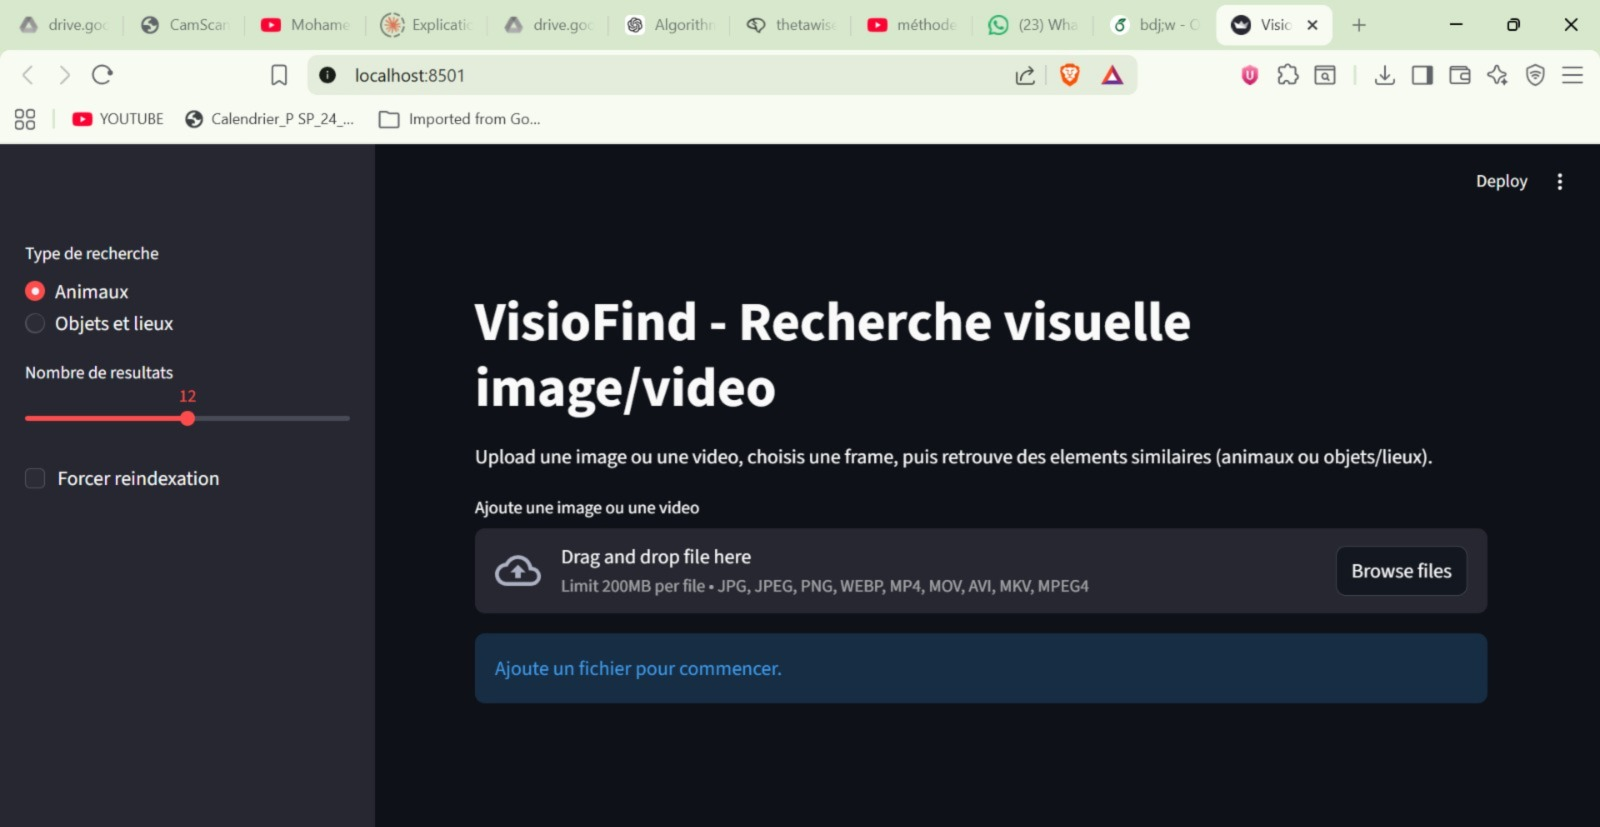
\includegraphics[width=0.92\textwidth]{t1_animaux_01_sidebar.jpeg}
  \caption{Interface — barre latérale en mode \emph{Animaux}~: choix du type de recherche, nombre de résultats (\texttt{top\_k}) et option de réindexation forcée.}
  \label{fig:t1a}
\end{figure}

\begin{figure}[htbp]
  \centering
  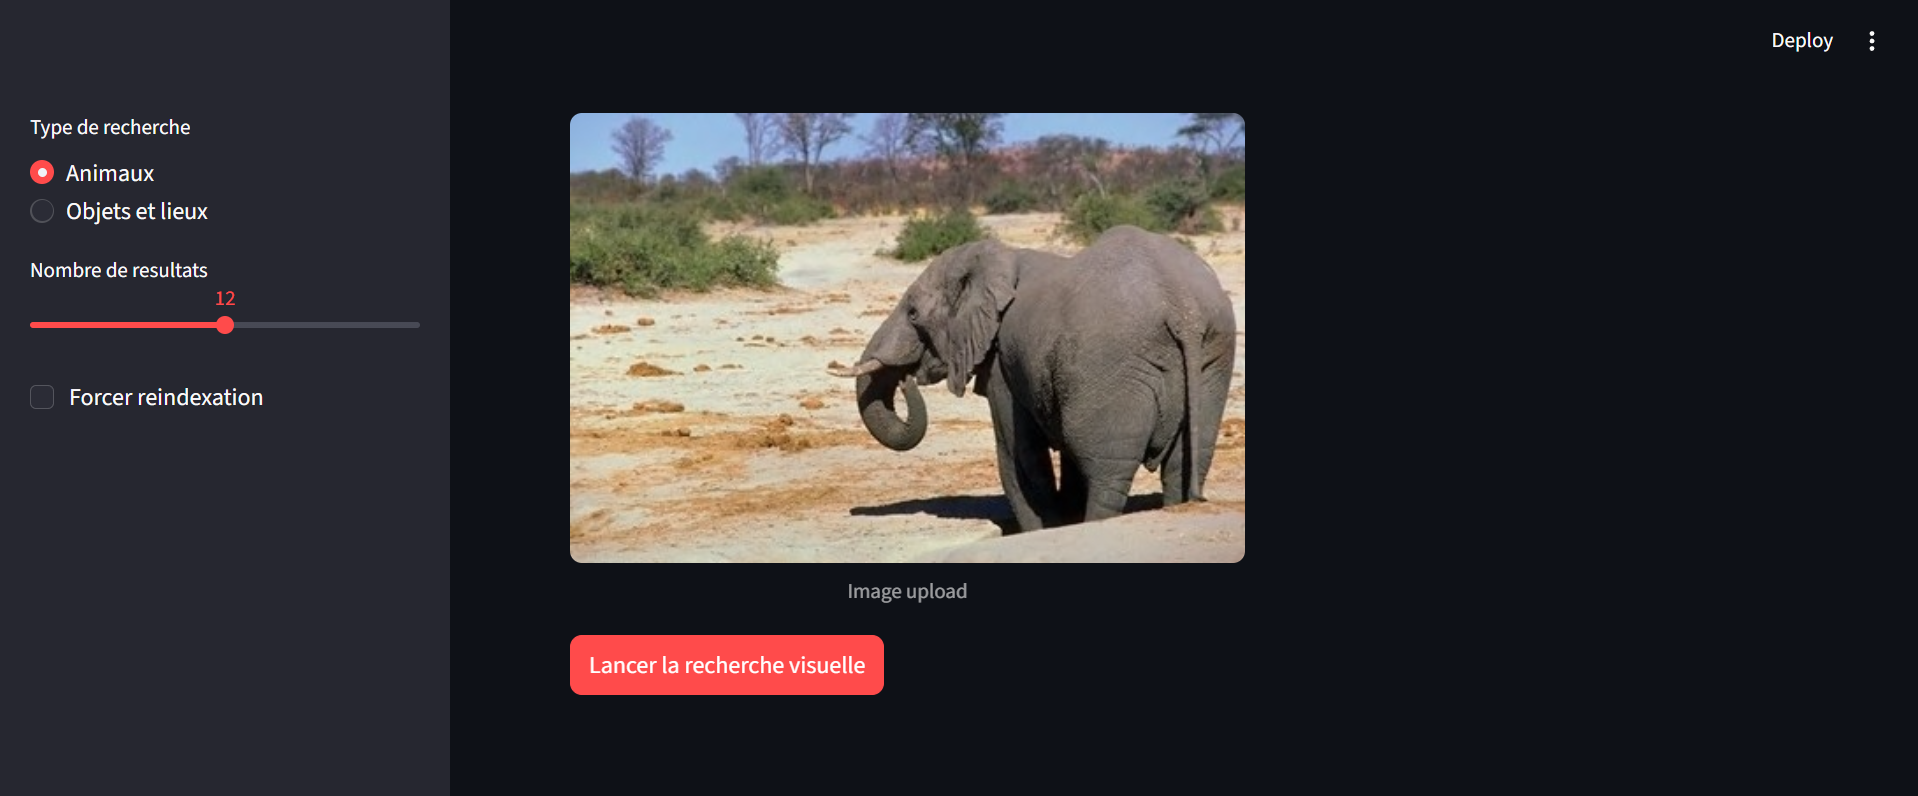
\includegraphics[width=0.92\textwidth]{t1_animaux_02_upload.png}
  \caption{Étape d'upload — téléversement de l'image de requête et aperçu avant lancement de la recherche visuelle.}
  \label{fig:t1b}
\end{figure}

\begin{figure}[htbp]
  \centering
  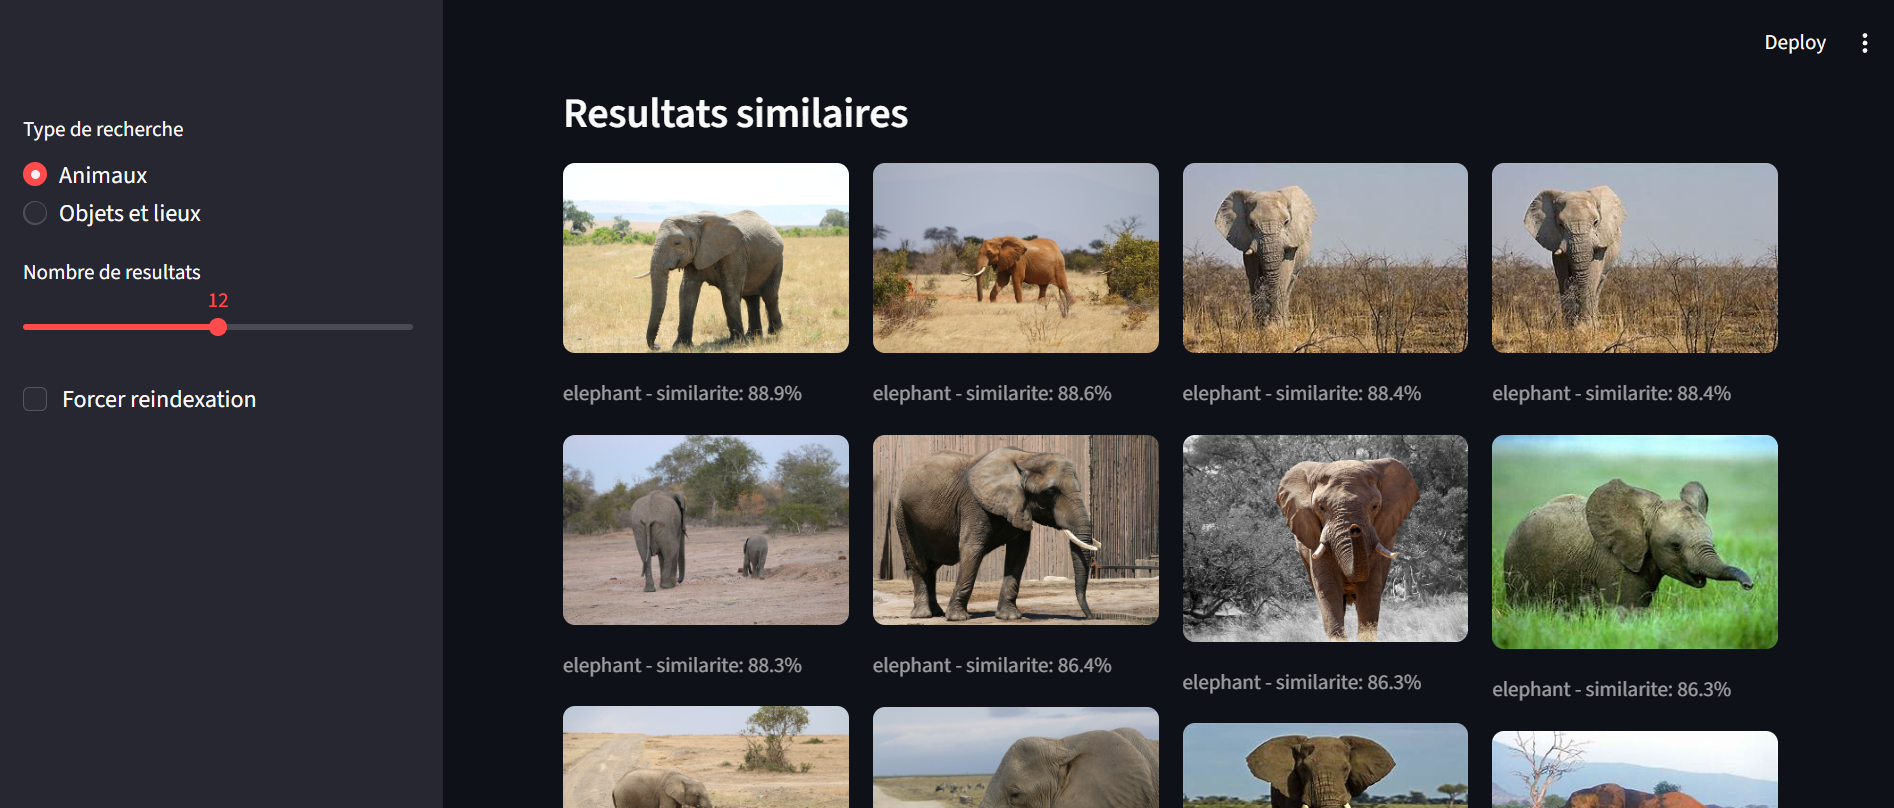
\includegraphics[width=0.92\textwidth]{t1_animaux_03_resultats.png}
  \caption{Résultats — mode \emph{Animaux}~: grille des images les plus similaires avec scores (pourcentage) et noms de classes issus de la structure de dossiers.}
  \label{fig:t1c}
\end{figure}

\section{Mode objets et lieux}

\begin{figure}[htbp]
  \centering
  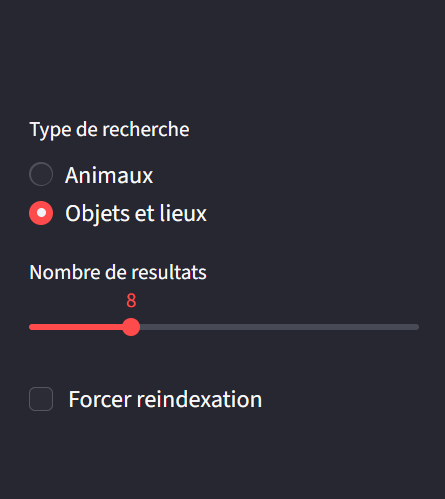
\includegraphics[width=0.92\textwidth]{t2_lieux_01_sidebar.png}
  \caption{Interface — passage au mode \emph{Objets et lieux} pour interroger la seconde galerie de référence.}
  \label{fig:t2a}
\end{figure}

\begin{figure}[htbp]
  \centering
  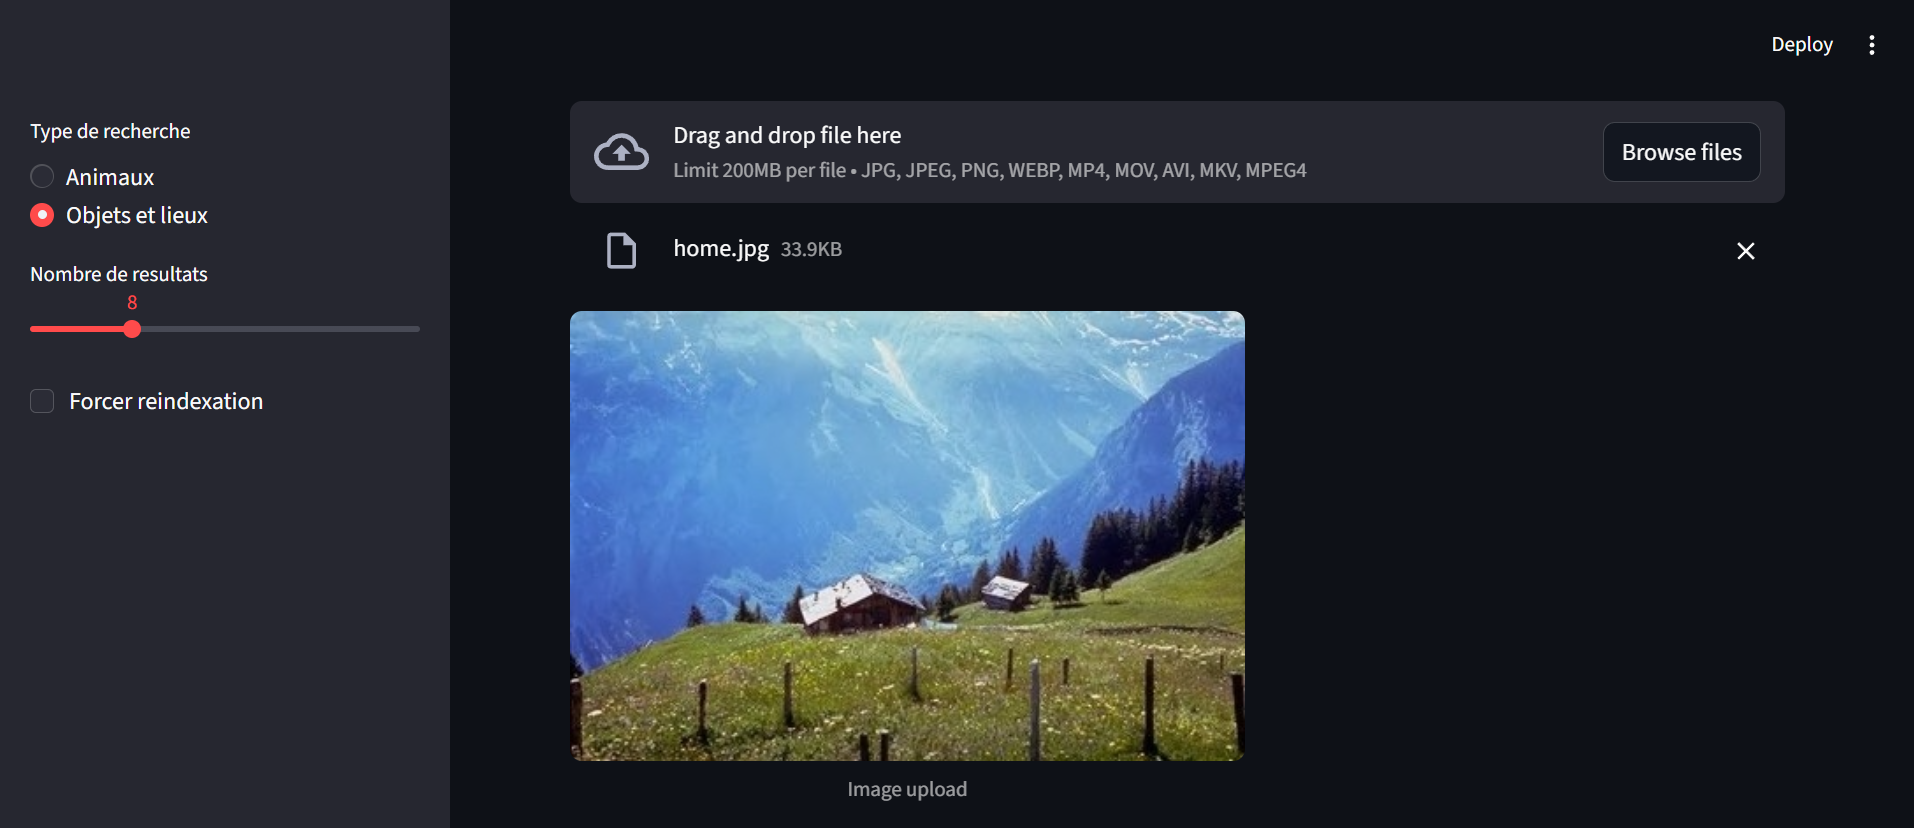
\includegraphics[width=0.92\textwidth]{t2_lieux_02_upload.png}
  \caption{Upload — image de requête représentative d'objets ou de scènes / lieux.}
  \label{fig:t2b}
\end{figure}

\begin{figure}[htbp]
  \centering
  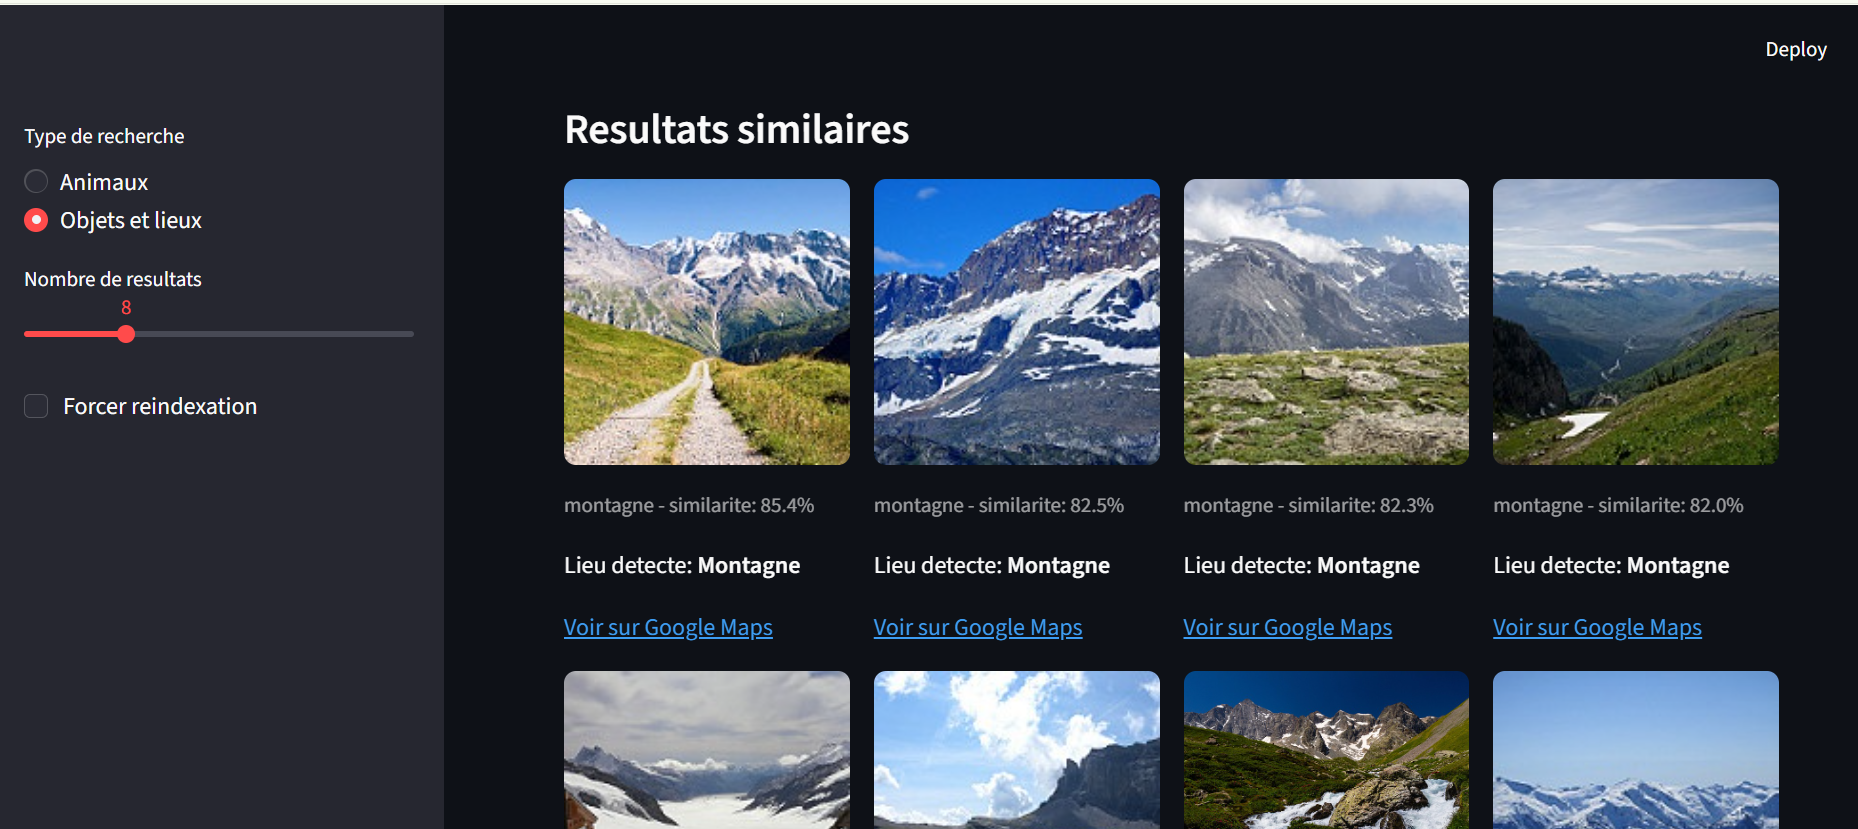
\includegraphics[width=0.92\textwidth]{t2_lieux_03_resultats_.png}
  \caption{Résultats — similarité visuelle dans la galerie \texttt{objets\_lieux} (scores et étiquettes de dossiers).}
  \label{fig:t2c}
\end{figure}

\begin{figure}[htbp]
  \centering
  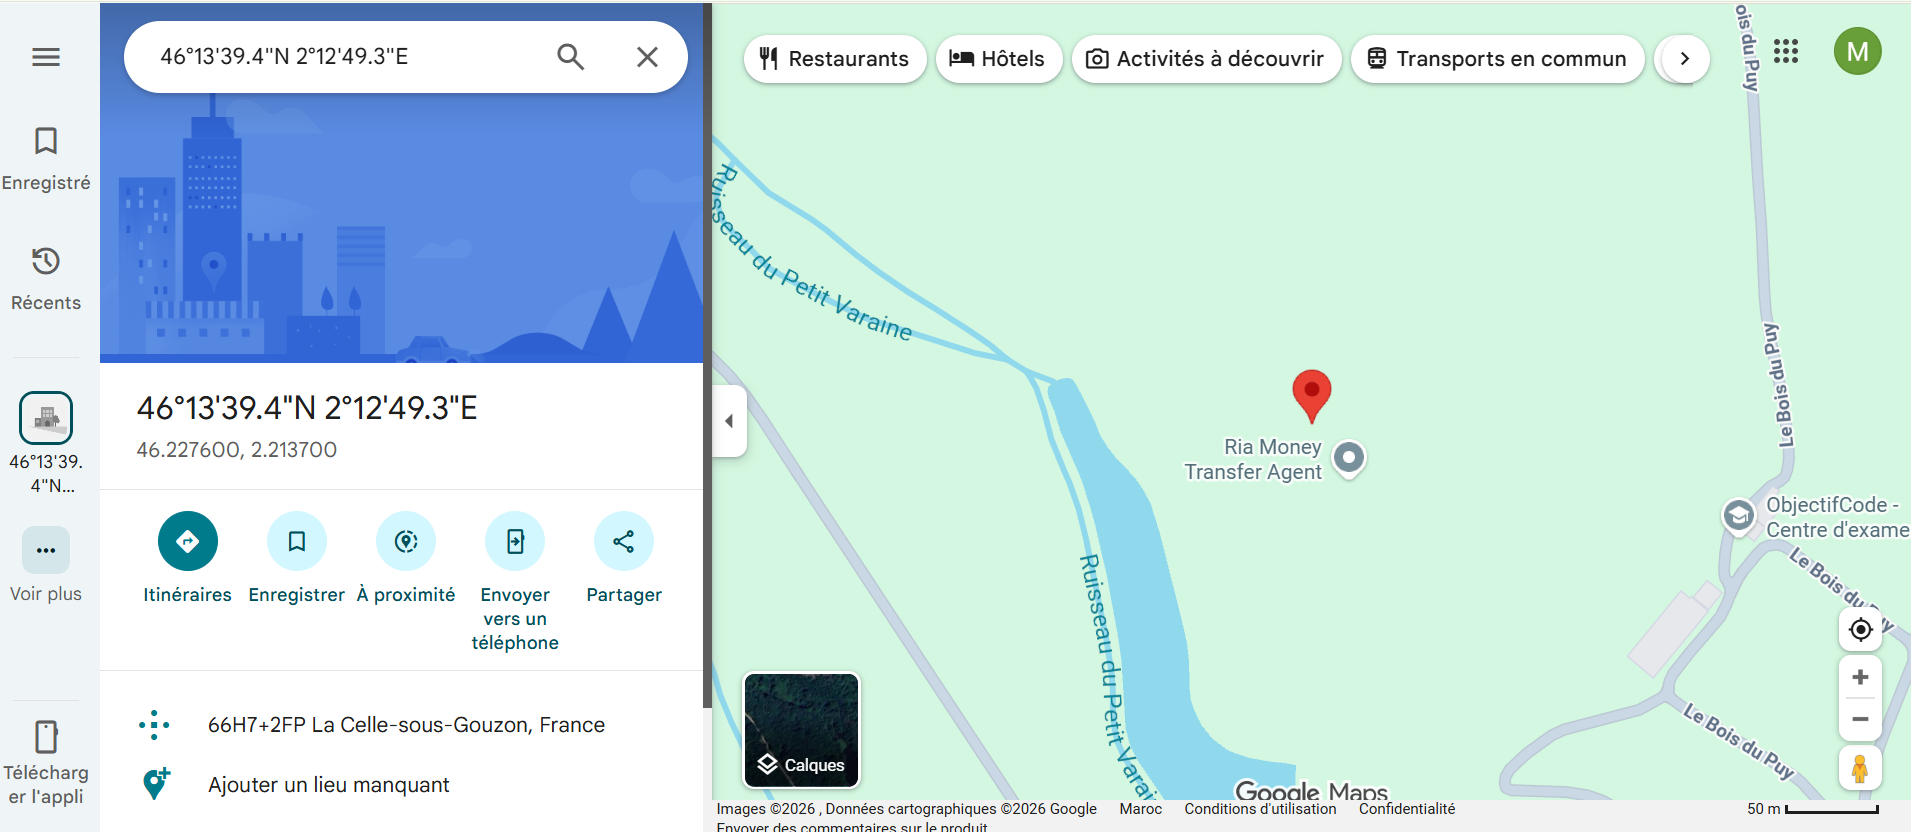
\includegraphics[width=0.92\textwidth]{t2_lieux_04_maps.png}
  \caption{Intégration cartographique — lorsque l'étiquette du résultat figure dans \texttt{KNOWN\_PLACES}, affichage du lieu et lien \emph{Google Maps}.}
  \label{fig:t2d}
\end{figure}

\paragraph{Note méthodologique.} Les captures proviennent du répertoire \texttt{docs/screenshots/} du projet. Le document accepte une compilation depuis \texttt{docs/} \emph{ou} depuis la racine du projet grâce à plusieurs chemins déclarés dans \texttt{\textbackslash graphicspath}.

% =============================================================================
% 14. RECHERCHE VIDÉO
% =============================================================================
\chapter{Recherche vidéo}

\section{Motivation de la fonctionnalité}

Une vidéo encode une \textbf{séquence temporelle} d'informations. Une frame isolée, choisie arbitrairement au début du clip, peut être floue, sous-exposée ou hors sujet. La fonctionnalité vidéo de VisioFind répond au besoin de \textbf{sélectionner l'instant pertinent} avant la recherche, ce qui rapproche le prototype des usages réels (archives touristiques, vidéos de surveillance amateur, contenus éducatifs).

\section{Principe — extraction des frames}

OpenCV ouvre le flux vidéo, lit les trames séquentiellement, et enregistre une image sur disque tous les \texttt{every\_n\_frames} (valeur par défaut 15), jusqu'à \texttt{max\_frames} (24). L'interface Streamlit liste les fichiers générés et un \texttt{selectbox} permet la sélection. Seule la frame choisie est passée au pipeline CLIP.

\section{Importance dans la vie réelle}

La navigation par \emph{keyframes} est un paradigme classique en indexation vidéo. Pour un utilisateur non expert, choisir une image représentative est souvent plus simple que de formuler une requête textuelle sur le contenu dynamique. Les limites actuelles (échantillonnage régulier, pas d'analyse sémantique temporelle) ouvrent des perspectives de recherche (détection de plans, résumé vidéo).

% =============================================================================
% 15. APPLICATIONS QUOTIDIENNES
% =============================================================================
\chapter{Applications dans la vie quotidienne}

\begin{itemize}[leftmargin=*]
  \item \textbf{Organisation de albums personnels}~: retrouver des clichés «~ressemblant à cette photo~» sans étiquetage manuel exhaustif.
  \item \textbf{Commerce et design}~: inspiration visuelle, recherche de produits analogues (dans une version industrielle couplée à un catalogue).
  \item \textbf{Éducation et musées}~: médiation numérique, parcours guidés par similarité visuelle.
  \item \textbf{Prototypage recherche}~: base de code pour expérimenter FAISS, fine-tuning ou multimodalité texte–image.
\end{itemize}

% =============================================================================
% 16. CONTRAINTES ET DIFFICULTÉS
% =============================================================================
\chapter{Contraintes et difficultés}

\section{Problèmes matériels}

Les machines sans \textbf{GPU} subissent des temps d'inférence CLIP plus longs, surtout lors de la première construction d'index. La \textbf{RAM} limite le batch d'images chargées simultanément lors du \texttt{build\_index}. Le \textbf{disque} doit accueillir le corpus et les caches.

\section{Dataset volumineux}

Au-delà de quelques milliers d'images, le scan linéaire et l'absence d'index vectoriel spécialisé (FAISS) deviennent des goulots d'étranglement. La maintenance d'un corpus hétérogène (doublons, images corrompues) demande des scripts de validation.

\section{Temps de calcul}

Le premier téléchargement des poids CLIP depuis Hugging Face dépend de la bande passante. Chaque session avec réindexation forcée reproduit le coût complet d'encodage.

\section{Limitations techniques diverses}

Blocages réseau (DuckDuckGo), configuration Kaggle sous Windows (fichier \texttt{kaggle.json} mal nommé), évolutions de l'API \texttt{transformers}, et comportement de Streamlit avec de très grandes images uploadées.

% =============================================================================
% 17. LIMITES DU PROJET
% =============================================================================
\chapter{Limites du projet}

\section{Précision}

Sans fine-tuning, CLIP peut confondre des classes fines (races, espèces proches) ou des scènes ambiguës. Les scores de cosinus ne sont pas des probabilités calibrées sur un jeu de labels du projet.

\section{Performance}

Complexité $\mathcal{O}(N)$ par requête en nombre d'images indexées. Pas de parallélisation multi-GPU ni de sharding des données.

\section{Généralisation}

Les biais du pré-entraînement (géographie, culture visuelle dominante) se répercutent sur les embeddings. Une galerie de référence déséquilibrée skew les résultats du top-$k$.

% =============================================================================
% 18. PERSPECTIVES D'AMÉLIORATION
% =============================================================================
\chapter{Perspectives d'amélioration}

\begin{itemize}[leftmargin=*]
  \item \textbf{Indexation approximative} (FAISS, ScaNN) pour le passage à l'échelle.
  \item \textbf{Fine-tuning} contrastif ou adaptation légère (\emph{adapter} layers) sur un domaine ciblé.
  \item \textbf{Segmentation / détection} préalable pour encoder des régions d'intérêt.
  \item \textbf{Géolocalisation réelle} à partir des métadonnées EXIF lorsqu'elles existent.
  \item \textbf{API REST} et conteneurisation Docker pour le déploiement.
  \item \textbf{Évaluation quantitative} (précision@$k$, protocole de requêtes annotées).
\end{itemize}

% =============================================================================
% 19. CONCLUSION GÉNÉRALE
% =============================================================================
\chapter{Conclusion générale}

VisioFind illustre de bout en bout une chaîne moderne de \textbf{recherche visuelle par contenu}~: constitution d'un corpus structuré, encodage par un modèle profond pré-entraîné multimodal (CLIP), persistance d'index, interface web interactive, extension vidéo par frames, et enrichissement cartographique pour des classes de lieux déclaratives. Le projet met en lumière les \textbf{atouts} des embeddings généralistes tout en rappelant les \textbf{limites} — performance en CPU, absence de segmentation, biais de données — et les \textbf{pistes} classiques d'un système de production (index rapide, spécialisation du modèle, évaluation rigoureuse). Sur le plan pédagogique, il constitue une passerelle tangible entre les concepts d'apprentissage profond, de traitement d'image et d'ingénierie logicielle web.

% =============================================================================
% ANNEXES (approfondissement — volume de pages pour rapport complet)
% =============================================================================
\appendix

\chapter{Guide d'installation, de configuration et d'exécution}

\section{Environnement Python}

Il est fortement recommandé d'isoler les dépendances dans un environnement virtuel. Sous Windows, depuis la racine du projet~:

\begin{lstlisting}
python -m venv .venv
.venv\Scripts\activate
pip install -r requirements.txt
\end{lstlisting}

Si une ancienne dépendance \texttt{duckduckgo-search} était installée, la migration vers \texttt{ddgs} s'effectue par désinstallation puis réinstallation conformément au fichier \texttt{README.md}.

\section{Lancement de l'application}

\begin{lstlisting}
streamlit run app.py
\end{lstlisting}

En cas d'absence de la commande \texttt{streamlit} dans le \texttt{PATH} (environnement virtuel non activé), utiliser~:

\begin{lstlisting}
python -m streamlit run app.py
\end{lstlisting}

\section{Constitution initiale de la galerie}

Avant une démonstration publique, exécuter par exemple~:

\begin{lstlisting}
python scripts/build_dataset.py --preset extended --per-class 120
\end{lstlisting}

Les images sont réparties sous \texttt{data/reference/animaux/} et \texttt{data/reference/objets\_lieux/}. Après ajout manuel massif, cocher \textbf{Forcer réindexation} dans l'interface pour invalider le cache et recalculer les embeddings.

\section{Authentification Kaggle (optionnel)}

Placer le fichier \texttt{kaggle.json} dans le dossier caché \texttt{.kaggle} du répertoire personnel Windows (par exemple \texttt{C:\textbackslash Users\textbackslash NomUtilisateur\textbackslash .kaggle\textbackslash}), en veillant à ce que le fichier ne soit pas enregistré sous le nom erroné \texttt{kaggle.json.txt}. La commande \texttt{python scripts/check\_kaggle\_auth.py} permet un diagnostic rapide.

\chapter{Compléments techniques et éthiques}

\section{Métriques d'évaluation en CBIR}

En recherche académique, on évalue souvent un système CBIR par la \textbf{précision@$k$} (proportion de résultats pertinents parmi les $k$ premiers) ou le \textbf{rappel} sur un jeu de requêtes pour lequel la vérité terrain (images pertinentes) a été annotée. VisioFind n'implémente pas encore ce protocole~; son intégration constitue une piste d'amélioration méthodologique majeure.

\section{Indexation approximative}

Lorsque $N$ dépasse le million de vecteurs, le produit scalaire exhaustif devient coûteux. Des bibliothèques comme \textbf{FAISS} (Facebook AI Similarity Search) proposent des structures de données (HNSW, IVF) qui échangent une légère imprécision contre un gain de temps dramatique. La migration consisterait à sérialiser les embeddings au format attendu par FAISS et à remplacer l'appel \texttt{np.dot} + \texttt{argsort} par une recherche de voisins approximatifs.

\section{Données, vie privée et propriété intellectuelle}

La collecte automatisée d'images depuis le Web soulève des questions de \textbf{copyright} et de \textbf{consentement}. Pour un usage institutionnel, il convient de privilégier des corpus sous licence ouverte, d'obtenir des autorisations, ou de produire ses propres photographies. Côté vie privée, tout déploiement traitant des données personnelles devrait respecter le RGPD et les politiques locales (anonymisation, durée de conservation, droit à l'effacement).

\section{Pistes de reproductibilité expérimentale}

Pour renforcer la rigueur scientifique du projet, on peut figer les versions exactes des paquets (\texttt{pip freeze}), documenter le matériel (CPU, RAM, présence GPU), et journaliser les temps d'indexation et de requête en fonction de $N$ et de $k$.

% =============================================================================
% 20. BIBLIOGRAPHIE
% =============================================================================
\cleardoublepage
\addcontentsline{toc}{chapter}{Bibliographie}

\begin{thebibliography}{99}

\bibitem{radford2021clip}
Radford, A., Kim, J.~W., Hallacy, C., Ramesh, A., Goh, G., Agarwal, S., Sastry, G., Askell, A., Mishkin, P., Clark, J., Krueger, G., Sutskever, I.
\newblock \emph{Learning Transferable Visual Models From Natural Language Supervision.}
\newblock arXiv:2103.00020, 2021.
\newblock \url{https://arxiv.org/abs/2103.00020}

\bibitem{dosovitskiy2020vit}
Dosovitskiy, A., Beyer, L., Kolesnikov, A., Weissenborn, D., Zhai, X., Unterthiner, T., Dehghani, M., Minderer, M., Heigold, G., Gelly, S., Uszkoreit, J., Houlsby, N.
\newblock \emph{An Image is Worth 16x16 Words: Transformers for Image Recognition at Scale.}
\newblock arXiv:2010.11929, 2020.

\bibitem{he2016resnet}
He, K., Zhang, X., Ren, S., Sun, J.
\newblock \emph{Deep Residual Learning for Image Recognition.}
\newblock Proceedings of the IEEE Conference on Computer Vision and Pattern Recognition (CVPR), 2016.

\bibitem{redmon2016yolo}
Redmon, J., Divvala, S., Girshick, R., Farhadi, A.
\newblock \emph{You Only Look Once: Unified, Real-Time Object Detection.}
\newblock Proceedings of CVPR, 2016.

\bibitem{smeulders2000cbir}
Smeulders, A.~W.~M., Worring, M., Santini, S., Gupta, A., Jain, R.
\newblock \emph{Content-Based Image Retrieval at the End of the Early Years.}
\newblock IEEE Transactions on Pattern Analysis and Machine Intelligence, 22(12), 2000.

\bibitem{deng2009imagenet}
Deng, J., Dong, W., Socher, R., Li, L.-J., Li, K., Fei-Fei, L.
\newblock \emph{ImageNet: A Large-Scale Hierarchical Image Database.}
\newblock Proceedings of CVPR, 2009.

\bibitem{huggingface2024}
Wolf, T. et al.
\newblock \emph{Transformers: State-of-the-Art Natural Language Processing.}
\newblock Proceedings of EMNLP (demonstration), 2020.
\newblock Documentation CLIP~: \url{https://huggingface.co/docs/transformers}

\bibitem{streamlit}
Streamlit Inc.
\newblock \emph{Streamlit — A faster way to build and share data apps.}
\newblock \url{https://streamlit.io/}

\bibitem{paszke2019pytorch}
Paszke, A. et al.
\newblock \emph{PyTorch: An Imperative Style, High-Performance Deep Learning Library.}
\newblock Advances in Neural Information Processing Systems (NeurIPS), 2019.

\end{thebibliography}

\end{document}
